\documentclass[problems]{esg8012exam} 
  \usepackage{amsmath}
  \usepackage{amssymb}
  \usepackage{enumerate}
  \usepackage{graphicx}
  \usepackage{hyperref}
  \usepackage{siunitx}
  \providecommand{\uvec}[1]{{\hat{\bf{#1}}}}
  \usepackage{pgf,tikz}
  \usetikzlibrary{arrows}
  \usepackage{subfigure}
  %\usepackage{wrapfig}
  \newcommand{\subfigureautorefname}{\figureautorefname}
  \makeatletter
  \newcommand{\interitemtext}[1]{%
    \begin{list}{}
    {\itemindent=0mm\labelsep=0mm
    \labelwidth=0mm\leftmargin=0mm
    \addtolength{\leftmargin}{-\@totalleftmargin}}
      \item #1
    \end{list}
  }
  \renewcommand{\d}{\,d}
  \providecommand{\norm}[1]{\lVert#1\rVert}
\classname{Physics 8.012} 
\semester{Fall 2010} 
\examnumber{2} 
\date{\today } 
\begin{document}
\bigskip 
\noindent \textbf {Name}\qquad \underline {\hspace {0.5\textwidth }}
\par 
\bigskip 
\noindent 
\textbf {The following exam consists of three problems. Answers without work shown will not be given any credit. Good luck!}
\par 
\bigskip 
\bigskip 
\bigskip 
\noindent \begin {tabular}{l@{\hspace {2em}}l@{\hspace {3em}}l}
\textbf {Problem 1} & \textbf {(30\space Points)} & \underline {\hspace {10em}} \\ \\ \\
\textbf {Problem 2} & \textbf {(35\space Points)} & \underline {\hspace {10em}} \\ \\ \\
\textbf {Problem 3} & \textbf {(35\space Points)} & \underline {\hspace {10em}} \\ \\ \\
\\ \\
\textbf {Total} & \textbf {(100\space Points)} & \underline {\hspace {10em}} \\ \\ \\
\end {tabular}
\cleardoublepage \relax 
\section{Problem \thesection\space(30\space points)}
  A block of mass $m_b$ sits at rest on a frictionless table; the block has a circular surface of radius $R$ as shown in the figure. A small cube of mass $m_c$ and speed $v_{c,0}$ is incident upon the block; the cube slides without friction on the table and slides without friction up the block. At the top of the block, the cube compresses a spring of spring constant $k$ until it momentarily comes to rest a height $R$ above the table. The cube then slides back down until it leaves the block.
  \begin{center}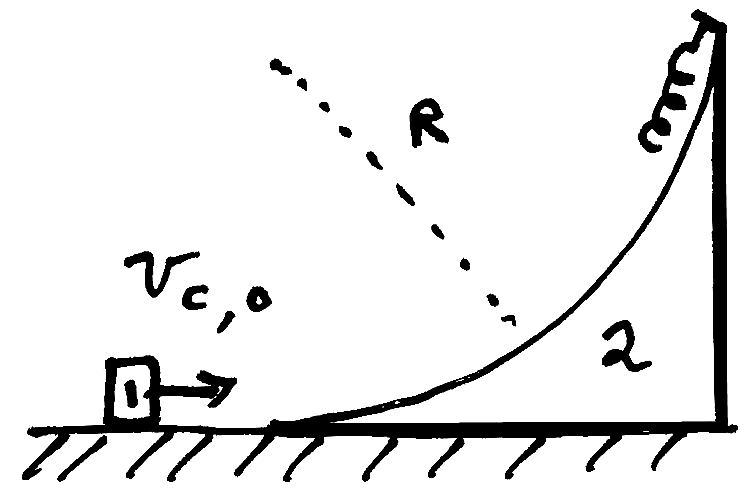
\includegraphics[width=0.35\textwidth]{exam2_p1_1}\end{center}
  \begin{enumerate}[(a)]
    \item How much did the spring compress?
    \item What is the final speed of the block when the cube is no longer on it?
  \end{enumerate}
\section{Problem \thesection\space(35\space points)}
  A particle initially sits on top of a large smooth sphere of radius $R$ as shown in the figure. The particle begins to slide along the surface of the sphere. There is a friction force between the particle and the surface that varies with the angle $\theta$ according to
  $$f = f_0\sin\theta$$
  where $f_0$ is a constant. Let $g$ denote the gravitational constant.
  \begin{center}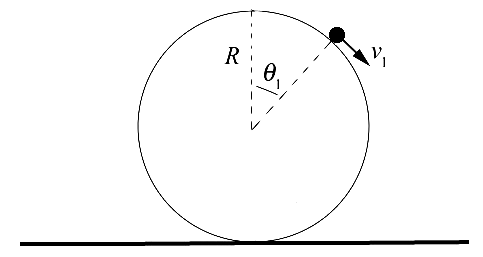
\includegraphics[width=0.4\textwidth]{exam2_p2_1}\end{center}
  \begin{enumerate}[(a)]
    \item Determine the angle $\theta_1$ with respect to the vertical at which the particle will lose contact with the surface of the sphere.
    \item What is the speed $v_1$ of the particle at the instant it loses contact with the surface of the sphere.
  \end{enumerate}
\par \vfil \penalty -\@M \write \m@ne {}\vbox {}\penalty -\@Mi \hbox {}\par \vfil \penalty -\@M 
\section{Problem \thesection\space(35\space points)}
  \begin{center}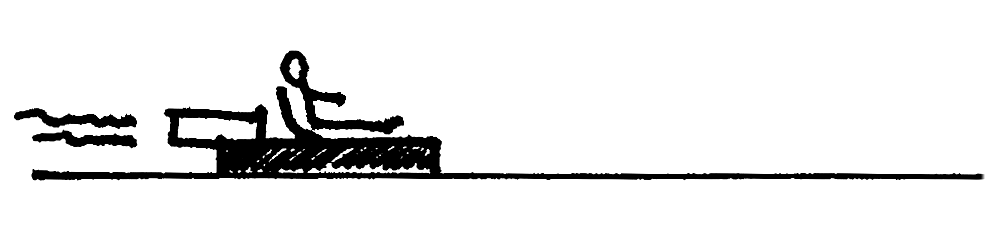
\includegraphics[width=0.6\textwidth]{exam2_p3_1}\end{center}
  A rocket sled ejects gas backwards at a speed $u$ relative to the rocket sled. The mass of the fuel in the rocket sled is equal to one half the initial total mass $m_{r,0}$ (including fuel) of the sled.  The rocket sled starts from rest on a frictionless track. You may ignore air resistance.
  \begin{enumerate}[(a)]
    \item Derive a relation between the differential of the speed of the rocket sled, $dv$, and the differential of the total mass of the rocket, $dm_r$.
    \item Integrate the above relation to find the speed of the rocket sled as a function of mass, $v_r(m)$, as the rocket sled speeds up.
    \item What is the final speed of the rocket sled after all the fuel has been burned?  Express your answers in terms of the quantities $u$, and $m_{r,0}$ as needed.
    \item After reaching its final speed, the sled enters a rough portion of the track that begins at $x=0$ with a coefficient of kinetic friction that varies with distance $\mu_k(x) = bx$ where $b$ is a positive constant.  How far $D$ did the sled slide before it came to rest in that portion of the track? Express your answers in terms of the quantities $u$, $b$, and $m_0$ as needed.
  \end{enumerate}
\end{document}
